% Section 06 - Manipulate Conductivity in Quantum Hall Systems

To identify the longitudinal conductivity characteristics of quantum Hall system under external dressing field, first we derive an expression for normalized longitudinal conductivity as a function of Fermi energy $X_F$ and intensity of the dressing field $I$.
We can identifiy the normalized $x$-directional longitudinal conductivity of dressed quantum Hall system by
\begin{equation}\label{eq:37}
  \widetilde{\sigma}^{xx}(X_F,I) =
  \flatfrac{\sigma^{xx}}{\sigma_{0}},
\end{equation}
with $\sigma^0 = \flatfrac{e^2}{(\pi \hbar A)}$, and this can be expressed as
\begin{equation} \label{eq:38}
  \begin{aligned}
    \widetilde{\sigma}^{xx}(X_F,I) &=
    \sum_{n}
    \frac{(n+1)}{\alpha^2 \Lambda_n \Lambda_{n+1}} \\
    &\quad\times
    \left[
      \frac{1}
      {
        1 + \left(\frac{X_F - n -1}{\alpha \Lambda_n}\right)^2
      }
    \right]
    \left[
      \frac{1}
      {
        1 + \left(\frac{X_F - n}{\alpha \Lambda_{n+1}}\right)^2
      }
    \right],
  \end{aligned}
\end{equation}
where $\alpha = \flatfrac{\Gamma_0}{(2\hbar \omega_0)}$. Here, $\Gamma_0$ is the natural energy broadening of the least Landau level.

As illustrated in Fig.~\ref{fig:5} and \ref{fig:6}, we can manipulate the normalized longitudinal conductivity $\widetilde{\sigma}^{xx}$ with the applied dressing field's intensity and the Fermi level $X_F$ of the considered system.
For a given dressing field intensity, the longitudinal conductivity varies with  the Fermi level of the system showing sharp peaks at each Landau energy level.
In quantum Hall systems, electrons are restricted to bear only the Landau energies. Thus, the conductivity reduces significantly when the Fermi level is not aligned with any of the Landau levels. In contrast, near each Landau level, the conductivity achieves excessive values compared to other areas. Moreover, as illustrates in Fig.~\ref{fig:5}, the peak value of the normalized longitudinal conductivity on each Landau level gets increase with the Landau level number.

On the other hand, considering the effects of the applied dressing field on the longitudinal conductivity of 2DEG, we can identify that the dressing field has sharpen the conductivity peaks.
When we increase the intensity level of the dressing field, the conductivity regions get more weaken as illustrated in the Fig.~\ref{fig:6}.
However, the peak value of the conductivity at each Landau level has the same value as the undressed system. This demonstrates our ability to tune the width of the conductivity regions in these quantum Hall systems with the help of a dressing field.

These characteristics align well with the outcomes demonstrated by Dini \textit{et al.} \cite{dini16}.  As the authors remarked in that publication, since the Fermi level of the system can be changed with the applied gate voltage of the material, this can be utilized as a 2D switch for nanoscale optoelectronics applications. Controlling  the external dressing field's intensity allows us to fine-tune this switching mechanism for optimized performance.
However, we can distinguish that the shapes and behavior of the conductivity regions illustrated in Fig.~\ref{fig:5} and Fig.~\ref{fig:6} are generally incompatible with the results reported in Ref.~\cite{dini16}. This is due to the selection of the conventional longitudinal conductivity theory of 2DEG from Refs.~\cite{ando74_1,ando82}. The semi-elliptical conductivity regions are  illustrated in Refs.~\cite{dini16,ando74_1,ando82}, have less consistency with the experimentally observed data for Landau levels \cite{endo09}.
In our study of the transport properties of quantum Hall systems, we developed the conductivity expression starting from the Floquet-Drude conductivity \cite{wackerl20} and we achieved outcomes that align with the results depicted in Ref. \cite{endo09}.
The theory on the conductivity of quantum Hall systems in Ref.~\cite{endo09} provides an excellent agreement with the experimentally observed results in GaAs/AlGaAs 2DEG for the low magnetic field range.
However, they have not considered the tunability that can be achieved with a dressing field. In this analysis, we account for both the magnetic and dressing field effects that can affect the transport properties of 2DEG, leading to a more generalized theory. Thus in this study, we were able to demonstrate that using Floquet-Drude conductivity method, one can derive a more generalized mathematical model which fits better with experiment for the charge transport properties of quantum Hall systems.

\begin{figure}[t]
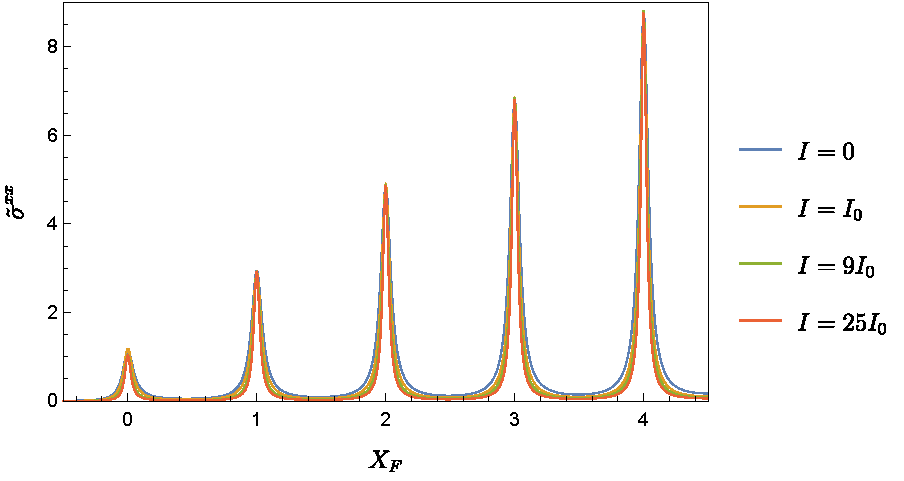
\includegraphics[scale=0.55]{figures/fig_4}
\caption{ Normalized longitudinal conductivity $\widetilde{\sigma}^{xx}$ against Fermi level $X_F$ with different intensities $I$ of the external dressing field in a GaAs-based quantum well under a nonoscillating magnetic field with $B = \SI{1.2}{\tesla}$, dressing field with a  frequency of $\omega =\SI{2e12}{\radian\per\second}$ and $I_0 =\SI{100}{\watt\per\square\centi\metre}$. In this calculation, we have assumed that the natural  broadening of $0$-th Landau level $\Gamma_0$ is $\SI{0.24}{\milli\eV}$.}
\label{fig:5}
\end{figure}

\begin{figure}[t]
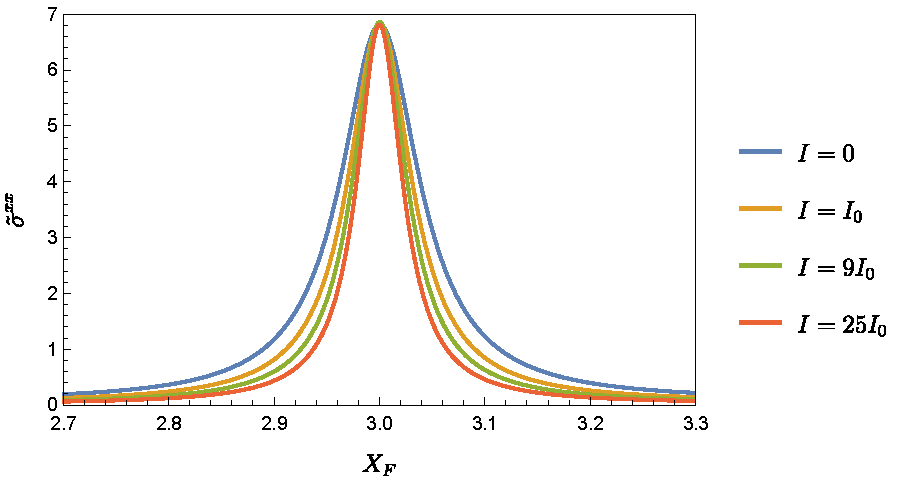
\includegraphics[scale=0.55]{figures/fig_5}
\caption{$3$rd Landau level’s normalized longitudinal conductivity $\widetilde{\sigma}^{xx}$ against Fermi level $X_F$ with different intensities $I$ of the external dressing field in a GaAs-based quantum well under a nonoscillating magnetic field with $B = \SI{1.2}{\tesla}$, dressing field with a frequency of $\omega =\SI{2e12}{\radian\per\second}$ and $I_0 =\SI{100}{\watt\per\square\centi\metre}$.
In this calculation, we have assumed that the natural  broadening of $0$-th Landau level $\Gamma_0$ is $\SI{0.24}{\milli\eV}$.}
\label{fig:6}
\end{figure}
